\documentclass[11pt,a4paper]{article}
\usepackage[T1]{fontenc}
\usepackage[margin=2.3cm]{geometry}
\usepackage{amsmath,amssymb}
\usepackage{graphicx}
\usepackage[dvipsnames]{xcolor}
\usepackage{enumitem}
\usepackage[colorlinks=true,linkcolor=blue,urlcolor=blue]{hyperref}
\setlength{\parskip}{0.6em}
\setlength{\parindent}{0pt}
\begin{document}

\begin{center}{\LARGE\bfseries opennutrition}\\[0.4em]{\large Balance food energy against activity, like a bank account, in three sessions.}\\[0.2em]\small PAN IIT OSS explainer \textbullet{} secondary school to diploma / undergraduate (levels 3-5)\end{center}

\section*{Why this exists}
Food carries energy and the body spends it all day. This explainer shows how to count that energy, how to estimate what a body uses, and why predictions about body mass are less certain than a simple rule suggests. It is general education, not medical or dietary advice.

\section*{The end goal}
Balance food energy against activity (general education, not medical advice). The end goal is to balance food energy against activity: to set up the bookkeeping, to model how mass responds, and to be honest about uncertainty. The same ideas of balance, steady states and error bars appear in engineering and science everywhere.

\section*{How the three sessions build up}
\begin{enumerate}[nosep]
\item \textbf{Session 1: Energy in, energy out: a bank balance} (Level 1, conceptual interactive model, 60 min).
\item \textbf{Session 2: Energy from nutrients, resting energy and a daily balance equation} (Level 2, mathematical engineering model, 75 min).
\item \textbf{Session 3: A dynamic model: mass approaches a steady state} (Level 3, simulation and validation, 90 min).
\end{enumerate}

\section{Session 1: Energy in, energy out: a bank balance}

\subsection*{A. Real-world problem}
Food carries energy and the body spends energy all day, even asleep. If more comes in than goes out the balance is positive; if less, it is negative, exactly like money in a bank account. Can we put numbers on a day and see the balance? This is general education only, not medical or dietary advice. The people are made up. Values for foods and activities are rounded textbook values and are approximate.

\subsection*{B. Concept and theory}
Energy is measured in kilocalories (kcal, also called Calories on food packs) or kilojoules (kJ): 1 kcal = 4.184 kJ. Energy in comes from food. Energy out is the energy the body spends on staying alive, moving and digesting. A common textbook estimate for activity is energy (kcal) = MET x body mass (kg) x time (hours), where a MET value says how many times the resting rate an activity uses; one MET is about one kcal per kg per hour. The daily balance is energy in minus energy out; adding balances day by day gives a running total, the account statement. All values are approximate and differ between people.

\begin{itemize}[nosep]
\item E\_in: energy in from food (kcal per day)
\item E\_out: energy out from the body and activities (kcal per day)
\item B: daily balance, E\_in - E\_out (kcal per day)
\item MET: activity intensity as a multiple of resting rate (no unit)
\item m: body mass (kg)
\item t: time spent on an activity (hours)
\end{itemize}

\begin{equation*}
1\ \mathrm{kcal}=4.184\ \mathrm{kJ}
\end{equation*}

\begin{equation*}
E_{\mathrm{out}}\approx\sum_{\text{activities}}\mathrm{MET}\times m\times t
\end{equation*}

\begin{equation*}
B = E_{\mathrm{in}}-E_{\mathrm{out}},\qquad \text{running total after } n \text{ days}=\sum_{i=1}^{n}B_i
\end{equation*}

\begin{center}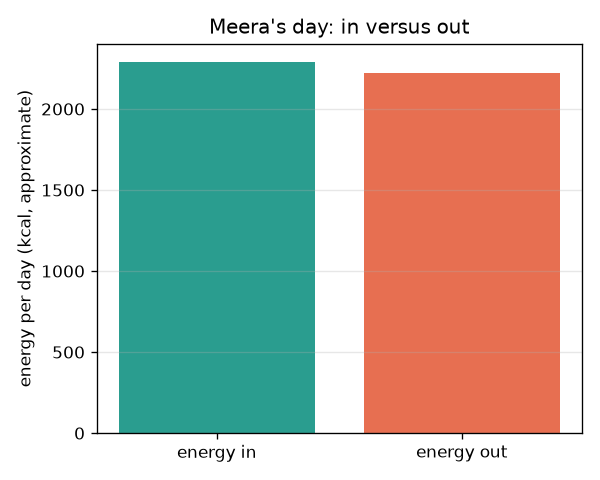
\includegraphics[width=0.85\linewidth]{figures/s01_day_bars.png}\\\small Meera's day: energy in against energy out (approximate values).\end{center}

\subsection*{E. Worked example}
How much energy does 1 hour of walking use for a 60 kg person, how many kilojoules is that, and how many bananas of food energy is it?
\begin{enumerate}[nosep]
\item Walking has MET 3.5 (approximate). Energy = 3.5 x 60 kg x 1 h = 210 kcal.
\item In kilojoules: 210 x 4.184 = 878.64, about 879 kJ.
\item One medium banana is about 105 kcal (approximate), so 210 / 105 = 2 bananas.
\end{enumerate}
\textbf{Answer.} About 210 kcal (about 879 kJ), roughly two bananas. All three numbers are approximate.

\subsection*{F. Questions}
\begin{enumerate}[nosep]
\item \textbf{Conceptual.} Meera sleeps and does nothing else for 8 hours. Is her energy out zero? Explain, and give the table estimate for a 60 kg person.
\item \textbf{Numerical.} A pack says 1500 kcal. How many kilojoules is that? Another day a person eats 2000 kcal and uses 2300 kcal: what is the balance and what is the running total after 7 days?
\item \textbf{Graph and simulation interpretation.} In the running-balance graph, what is the value of the '300 kcal short each day' line after 14 days, and what does the slope of a line mean?
\item \textbf{Design and optimisation challenge.} Meera's day gives a balance of +66 kcal. By swapping half an hour of sitting for walking, can she bring it to zero? Show the working and state the assumption.
\end{enumerate}

\section{Session 2: Energy from nutrients, resting energy and a daily balance equation}

\subsection*{A. Real-world problem}
A food label lists grams of protein, carbohydrate and fat and also a number of kilocalories. Do they agree? And how many kilocalories does a person use per day, so a day of meals can be balanced against a given activity plan? This is general education only, not medical or dietary advice. The people are made up. The formulas are population estimates and an individual can differ a lot.

\subsection*{B. Concept and theory}
Energy from food is estimated with general factors: 4 kcal per gram of protein, 4 per gram of carbohydrate and 9 per gram of fat. Printed labels use more detailed factors and rounding, so a small difference from the sum is normal. Resting energy (basal metabolic rate, BMR) can be estimated with the Mifflin-St Jeor equation: BMR = 10 m + 6.25 h - 5 a + s, with s = +5 for males and -161 for females. It was fitted to groups of people; for one person the real value can be quite different, so it is a starting guess, not a measurement. Total daily energy use (TDEE) is the BMR times an activity factor (PAL); common textbook values are 1.2, 1.375, 1.55 and 1.725 from sedentary to active. A rough short-term rule says that about 7700 kcal of surplus adds about 1 kg of body mass, giving the difference equation M[n+1] = M[n] + (I - E) / 7700 with I and E held constant. The body adapts when mass and activity change, so this rule is only a short-term approximation and worsens over longer times.

\begin{itemize}[nosep]
\item P, C, F: protein, carbohydrate and fat in a food (g)
\item m: body mass (kg)
\item h: height (cm)
\item a: age (years)
\item s: sex constant (+5 male, -161 female) (kcal/day)
\item PAL: activity factor (no unit)
\item I, E: energy in and energy used per day (kcal/day)
\item M[n]: body mass on day n (kg)
\end{itemize}

\begin{equation*}
E_{\mathrm{food}}=4P+4C+9F\quad(\mathrm{kcal};\ P,C,F\ \text{in g})
\end{equation*}

\begin{equation*}
\mathrm{BMR}=10\,m+6.25\,h-5\,a+s\quad(\mathrm{kcal/day})
\end{equation*}

\begin{equation*}
\mathrm{TDEE}=\mathrm{BMR}\times\mathrm{PAL}
\end{equation*}

\begin{equation*}
M[n+1]=M[n]+\frac{I-E}{7700}\quad\Rightarrow\quad \Delta M=\frac{(I-E)\,N}{7700}\ \text{after } N \text{ days}
\end{equation*}

\begin{center}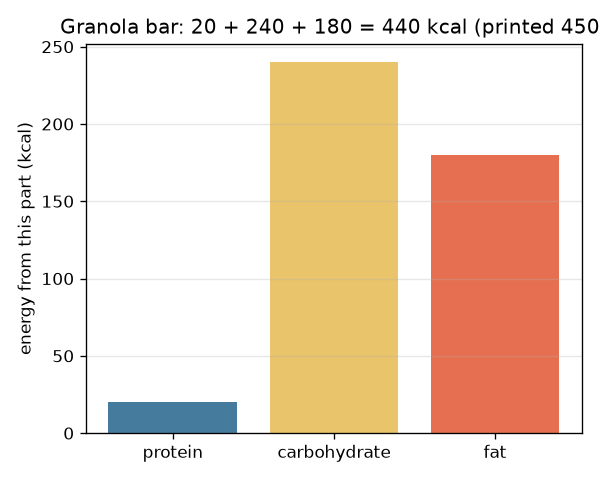
\includegraphics[width=0.85\linewidth]{figures/s02_label_parts.png}\\\small Granola bar: energy from protein, carbohydrate and fat sums to 440 kcal.\end{center}

\subsection*{E. Worked example}
Ravi (made up) is male, 19 years, 175 cm and 70 kg, with a moderate activity factor of 1.55. Find his BMR and TDEE. If he eats 2900 kcal a day for 30 days, what mass change does the 7700 rule give?
\begin{enumerate}[nosep]
\item BMR = 10 x 70 + 6.25 x 175 - 5 x 19 + 5 = 700 + 1093.75 - 95 + 5 = 1703.75 kcal/day.
\item TDEE = 1703.75 x 1.55 = 2640.8 kcal/day (rounded).
\item Surplus = 2900 - 2640.8 = 259.2 kcal/day.
\item Change after 30 days = 259.2 x 30 / 7700 = 1.01 kg (rough rule).
\end{enumerate}
\textbf{Answer.} BMR 1703.75 kcal/day, TDEE about 2640.8 kcal/day, and about +1.01 kg in 30 days by the rough rule.

\subsection*{F. Questions}
\begin{enumerate}[nosep]
\item \textbf{Conceptual.} Why is the 7700 kcal per kg rule only a short-term approximation?
\item \textbf{Numerical.} An energy bar label says 8 g protein, 30 g carbohydrate and 12 g fat, and prints 270 kcal. Compute the energy from grams and the difference. Is the label wrong?
\item \textbf{Graph and simulation interpretation.} In the 30-day graph the lines are straight. If a person's intake is 500 kcal above E, how much does the rule predict in 30 days and what is the slope?
\item \textbf{Design and optimisation challenge.} Design: choose servings from the menu (rice 205, dal 204, chapati 111, paneer 134, milk 152, banana 112, peanuts 178, egg 73 kcal per serving) for Ravi so that the day's food is within 50 kcal of his TDEE, uses at least 5 different items and at most 4 servings of any item. State one trade-off.
\end{enumerate}

\section{Session 3: A dynamic model: mass approaches a steady state}

\subsection*{A. Real-world problem}
Session 2 held energy use fixed. But a heavier body uses more energy, so a constant extra intake adds mass more and more slowly. How different is that from the straight-line rule, and how much can uncertain food logs and resting-energy estimates blur any prediction? This is general education only, not medical or dietary advice. The people are made up. This is a simplified model, not a clinical tool.

\subsection*{B. Concept and theory}
With Mifflin-St Jeor, energy use is a straight line in mass: E(M) = A M + B, where A = 10 x PAL kcal/day per kg and B = PAL x (6.25 h - 5 a + s) kcal/day. Treating mass as continuous, dM/dt = (I - A M - B) / 7700. This linear equation has an exact solution: M(t) = M\_ss + (M0 - M\_ss) exp(-t / tau), with steady state M\_ss = (I - B) / A and time constant tau = 7700 / A. Mass moves toward M\_ss and the speed is proportional to the distance still to go, so the curve flattens. A numerical Euler solution with a step of one day can be checked against this formula. The naive rule freezes E at its starting value and gives a straight line. Uncertainty: if logged intake and the BMR estimate are each off by up to 10 percent, many random draws (Monte Carlo) give a spread of outcomes. Simplifications: composition of tissue, water, hormones and behaviour are not modelled.

\begin{itemize}[nosep]
\item M: body mass (kg)
\item I: energy in per day (kcal/day)
\item A, B: slope and offset of expenditure E = A M + B (kcal/day per kg, kcal/day)
\item M\_ss: steady-state mass (kg)
\item tau: time constant (days)
\item dt: time step (days)
\end{itemize}

\begin{equation*}
E(M)=A\,M+B,\quad A=10\,\mathrm{PAL},\quad B=\mathrm{PAL}\,(6.25h-5a+s)
\end{equation*}

\begin{equation*}
\frac{dM}{dt}=\frac{I-A\,M-B}{7700}
\end{equation*}

\begin{equation*}
M(t)=M_{ss}+(M_0-M_{ss})\,e^{-t/\tau},\quad M_{ss}=\frac{I-B}{A},\quad \tau=\frac{7700}{A}
\end{equation*}

\begin{equation*}
M_{n+1}=M_n+\Delta t\,\frac{I-A\,M_n-B}{7700}\quad\text{(Euler)}
\end{equation*}

\begin{center}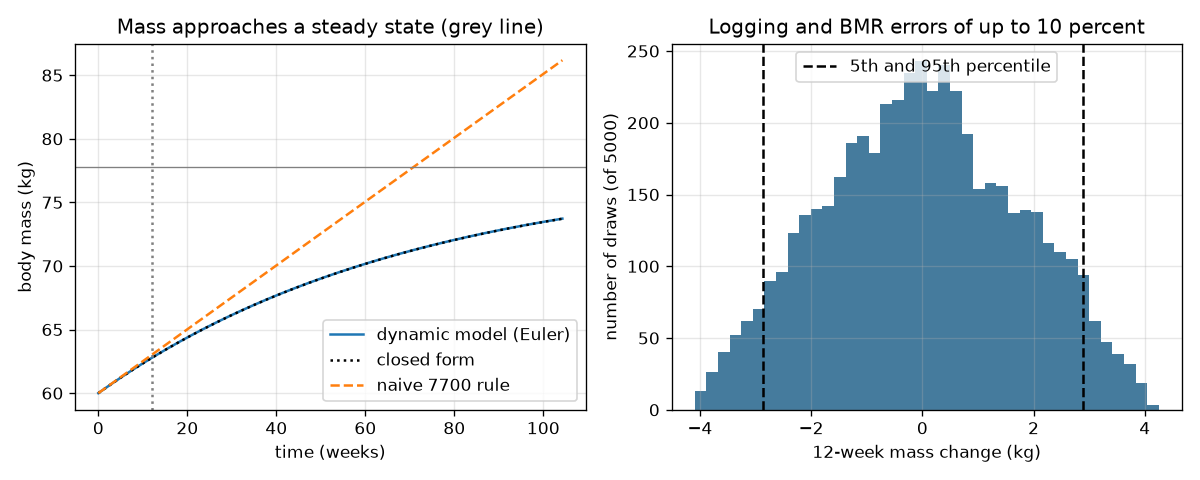
\includegraphics[width=0.85\linewidth]{figures/s03_dynamic_and_spread.png}\\\small Left: dynamic model, closed form and naive rule. Right: spread of the 12-week mass change from 10 percent errors.\end{center}

\subsection*{E. Worked example}
Asha (made up) is 60 kg, 165 cm, 20 years, female, PAL 1.55, and eats 2400 kcal a day. Find the steady state and the mass after 12 weeks (84 days) from the dynamic model and the naive rule.
\begin{enumerate}[nosep]
\item A = 10 x 1.55 = 15.5 kcal/day per kg. B = 1.55 x (6.25 x 165 - 5 x 20 - 161) = 1193.89 kcal/day.
\item Starting use E0 = 15.5 x 60 + 1193.89 = 2123.9 kcal/day, so the surplus is 2400 - 2123.9 = 276.1 kcal/day.
\item Steady state M\_ss = (2400 - 1193.89) / 15.5 = 77.81 kg. Time constant tau = 7700 / 15.5 = 497 days (rounded).
\item Dynamic after 84 days: 62.77 kg. Naive: 60 + 276.1 x 84 / 7700 = 63.01 kg.
\end{enumerate}
\textbf{Answer.} Steady state 77.81 kg. After 12 weeks the models differ only slightly: 62.77 kg (dynamic) against 63.01 kg (naive). After 2 years they differ a lot: 73.72 kg against 86.18 kg.

\subsection*{F. Questions}
\begin{enumerate}[nosep]
\item \textbf{Conceptual.} Why does the dynamic curve flatten while the naive line does not?
\item \textbf{Numerical.} For Asha, what steady-state mass does an intake of 2200 kcal a day give, and what fraction of the way to the steady state has the mass travelled after one time constant?
\item \textbf{Graph and simulation interpretation.} Reading the first figure: by how much do the naive and dynamic answers differ at 12 weeks and at 2 years (intake 2400)? What does this tell you about using the 7700 rule?
\item \textbf{Design and optimisation challenge.} Design: a planner for the made-up person Asha (sedentary base, 60 kg) wants a starting daily balance between -225 and -175 kcal using meal plans of 1400, 1500, 1600 or 1700 kcal and walking in 15 minute steps up to 1.5 hours. Which plans pass, which is the least walking, and can a 12-week weigh-in confirm it? State a trade-off.
\end{enumerate}

\section{Real-world mini-project}
\textbf{Plan a meal-and-walk schedule for a made-up person.} Asha (made up) is 20, 165 cm and 60 kg, with a sedentary day. A planner wants a starting daily balance between -225 and -175 kcal. Choose meal plans from 1400, 1500, 1600 and 1700 kcal a day and walking times from 0 to 1.5 hours in 15 minute steps, using \texttt{plan\_balance} from Session 3. Then simulate the best plan for 12 weeks and measure how far logging and BMR errors of up to 10 percent could move the result. This is a classroom exercise with a fictional person, not advice for anyone.

\section{The path ahead}
\begin{enumerate}[nosep]
\item \textbf{Session 4: Estimate the hidden intake bias from weigh-ins.} Simulate 8 weeks of daily weigh-ins with 0.5 kg noise for a person whose true intake is above the logged value, then estimate the bias by least squares.
\item \textbf{Session 5: Fat and lean compartments.} A two-compartment model of body composition replacing the single 7700 kcal per kg constant.
\item \textbf{Session 6: Rank the sources of uncertainty.} A variance-based sensitivity study of intake error, BMR error and portion size error.
\item \textbf{Session 7: Weekly schedules with weekends.} A model whose intake and walking differ between weekdays and weekends.
\item \textbf{Session 8: Reproduce the Target animation.} An animated GIF with the energy-in and energy-out bars, the mass curve, the naive line and a shaded band.
\end{enumerate}

\section{Answers and hints}

\subsection*{Session 1}
\begin{enumerate}[nosep]
\item \textbf{Conceptual.} Hint: Sleeping has a MET value just below 1. Solution: No. The body keeps working while asleep (heart, breathing, repair, keeping warm). With MET 0.95, energy = 0.95 x 60 x 8 = 456 kcal. Energy out is never zero, which is why the balance is not simply 'food minus exercise'.
\item \textbf{Numerical.} Hint: Multiply by 4.184, then multiply the daily balance by 7. Solution: 1500 x 4.184 = 6276 kJ. Balance = 2000 - 2300 = -300 kcal per day; after 7 days the running total is 7 x (-300) = -2100 kcal. Sanity check: the units are kcal and the sign is negative because less came in than went out.
\item \textbf{Graph and simulation interpretation.} Hint: Slope is rise over run: kcal per day. Solution: After 14 days the line is at 14 x (-300) = -4200 kcal. The slope of each line is the daily balance in kcal per day: steeper means a bigger daily surplus or shortfall, flat means balance.
\item \textbf{Design and optimisation challenge.} Hint: Walking uses 3.5 MET and sitting 1.3 MET; find the extra kcal per hour for 60 kg. Solution: Extra energy per hour of walking instead of sitting = (3.5 - 1.3) x 60 = 132 kcal. Half an hour gives 66 kcal. So her energy out rises from 2223 to 2289 kcal, which equals her 2289 kcal in, and the balance is zero. Assumption: the MET table is exact for her; in reality it is only an estimate, so the true balance is uncertain.
\end{enumerate}

\subsection*{Session 2}
\begin{enumerate}[nosep]
\item \textbf{Conceptual.} Hint: Think about what happens to the energy a body uses when its mass changes. Solution: The rule holds E constant. In reality when mass changes, resting energy changes with it, and activity and other processes adapt too, so the same daily surplus has a smaller and smaller effect. It is acceptable for a few days or weeks and becomes less reliable over longer times (Session 3).
\item \textbf{Numerical.} Hint: 4 x 8 + 4 x 30 + 9 x 12. Solution: 32 + 120 + 108 = 260 kcal. The label is 10 kcal above (10 / 270 = 3.7 percent). Not necessarily wrong: labels use detailed factors, fibre and rounding. A difference of a few percent is normal; a very large one would be worth a second look.
\item \textbf{Graph and simulation interpretation.} Hint: Slope = surplus / 7700 in kg per day. Solution: Change = 500 x 30 / 7700 = 1.95 kg. The slope is 500 / 7700 = 0.065 kg per day. Straight lines are a consequence of holding E constant.
\item \textbf{Design and optimisation challenge.} Hint: His TDEE is about 2640.8 kcal; try to add up around 2640. Solution: One valid plan: rice 2, dal 3, chapati 4, paneer 2, milk 2, banana 2, peanuts 2. Energy = 410 + 612 + 444 + 268 + 304 + 224 + 356 = 2618 kcal, which is 22.8 kcal below his TDEE and uses 7 items. Trade-off: this only balances energy; it ignores protein, fibre, vitamins, cost and taste, and Ravi's real needs depend on much more than a population formula.
\end{enumerate}

\subsection*{Session 3}
\begin{enumerate}[nosep]
\item \textbf{Conceptual.} Hint: What happens to energy used as mass rises? Solution: As mass rises, energy used rises (E = A M + B), so the gap I - E shrinks and mass changes more slowly. The naive rule freezes E at its starting value, so the gap never shrinks and the line stays straight. The curve flattens toward the steady state where E equals I.
\item \textbf{Numerical.} Hint: M\_ss = (I - B) / A; after one tau the remaining distance is multiplied by e\textasciicircum{}-1. Solution: M\_ss = (2200 - 1193.89) / 15.5 = 64.91 kg. After one time constant the mass has covered 1 - e\textasciicircum{}-1 = 0.632, that is 63.2 percent of the way. Sanity check: the units are kg and the answer lies between the 60 kg start and the 77.81 kg of the 2400 kcal case, as expected for a smaller intake.
\item \textbf{Graph and simulation interpretation.} Hint: Subtract the dynamic values from the naive values. Solution: At 12 weeks 63.01 - 62.77 = 0.24 kg; at 2 years 86.18 - 73.72 = 12.46 kg. The rule is a fair short-term approximation but becomes very misleading when extended over long times.
\item \textbf{Design and optimisation challenge.} Hint: Use plan\_balance, find\_plans, plan\_outcome and plan\_spread from the lesson. Solution: Passing plans: (1500 kcal, 0.25 h), (1500 kcal, 0.5 h) and (1600 kcal, 1.0 h). The least walking is 1500 kcal with 0.25 h: its starting balance is -181.8 kcal/day, the dynamic model predicts -1.85 kg in 12 weeks, but with 10 percent errors the 5th to 95th percentile spread is about -4.03 to +0.33 kg, so a 12-week weigh-in cannot confirm the plan. Trade-off: a bigger walk allows a larger meal, but takes more time; either way the uncertainty is larger than the effect. This is a classroom exercise, not advice.
\end{enumerate}

\section{How to join}
Read \texttt{CONTRIBUTING.md} in the repository, then pick an issue labelled \texttt{good first issue}. Repository: \url{https://github.com/KrunalPanchal1995/opennutrition}

\end{document}
